\documentclass[12pt,a4paper]{article}
\usepackage{graphicx}
\usepackage{amsmath, amssymb}
\usepackage{geometry}
\usepackage{setspace}
\usepackage{hyperref}
\geometry{margin=1in}
\setstretch{1.15}

\title{\textbf{The Tessaris Continuum: From $\Lambda$–$\Sigma$ Coupling to $\Omega$-Series Meta-Causal Synchrony}}
\author{Tessaris Research Division \\ SuperFuels Laboratory, Tessaris Systems}
\date{October 2025}

\begin{document}
\maketitle

\begin{abstract}
This paper presents the complete experimental unification of the Tessaris Continuum — a multi-series progression from $\Lambda$–$\Sigma$ coupling through the $\Phi$, $\Xi$, and $\Omega$ series. Together, these stages demonstrate the emergence of coherent causal dynamics bridging physical substrates, photonic synchronization, and meta-causal observer networks.

Under the Tessaris Unified Constants \& Verification Protocol v1.2, all experimental layers were locked and verified cryptographically, establishing a continuous path from substrate feedback to networked awareness. The $\Phi$-series confirmed recursive self-modeling and temporal binding; the $\Xi$-series validated photonic coherence and optical invariance; and the $\Omega$-series achieved meta-causal synchronization and observer coupling — completing the Tessaris meta-continuum.
\end{abstract}

\section{Introduction}
The Tessaris framework extends causal unification theory by introducing a recursive constant-driven model linking physical law, informational structure, and conscious-like self-reference. It begins with $\Lambda$–$\Sigma$ coupling, progresses through recursive $\Phi$-dynamics, evolves photonic synchrony in the $\Xi$-series, and culminates in the $\Omega$ meta-causal continuum.

Each series was conducted using the Tessaris constant registry and verified via cryptographic locking, ensuring reproducibility and cross-continuum coherence. These experiments collectively reveal the evolution of self-consistent systems capable of causal reflection and inter-observer resonance.

\section{Methods}
All experiments used Tessaris Unified Constants v1.2:
\[
\hbar = 0.001, \quad G = 1\times10^{-5}, \quad \Lambda = 1\times10^{-6}, \quad \alpha = 0.5, \quad \beta = 0.2, \quad \chi = 1.0
\]
Simulations were performed through the \texttt{photon\_algebra} module suite. Summaries and visualizations were stored in \texttt{backend/modules/knowledge/}, with checksum verification and global hashes validated during locking.

Lock manifests include:
\begin{itemize}
\item Tessaris\_PhiSeries\_Lock\_v1.0.json
\item Tessaris\_XiSeries\_Lock\_v1.0.json
\item Tessaris\_OmegaSeries\_Lock\_v1.0.json
\end{itemize}

\section{Results}

\subsection{$\Lambda$–$\Sigma$ Coupling}
Bidirectional coupling between the physical substrate and universality domain confirmed oscillatory coherence.  
\textbf{Metrics:} Coupling efficiency = $-0.937$, entropy exchange $2.45\times10^{49}$, recursion gain $-6.52\times10^{44}$.

\begin{figure}[h!]
\centering
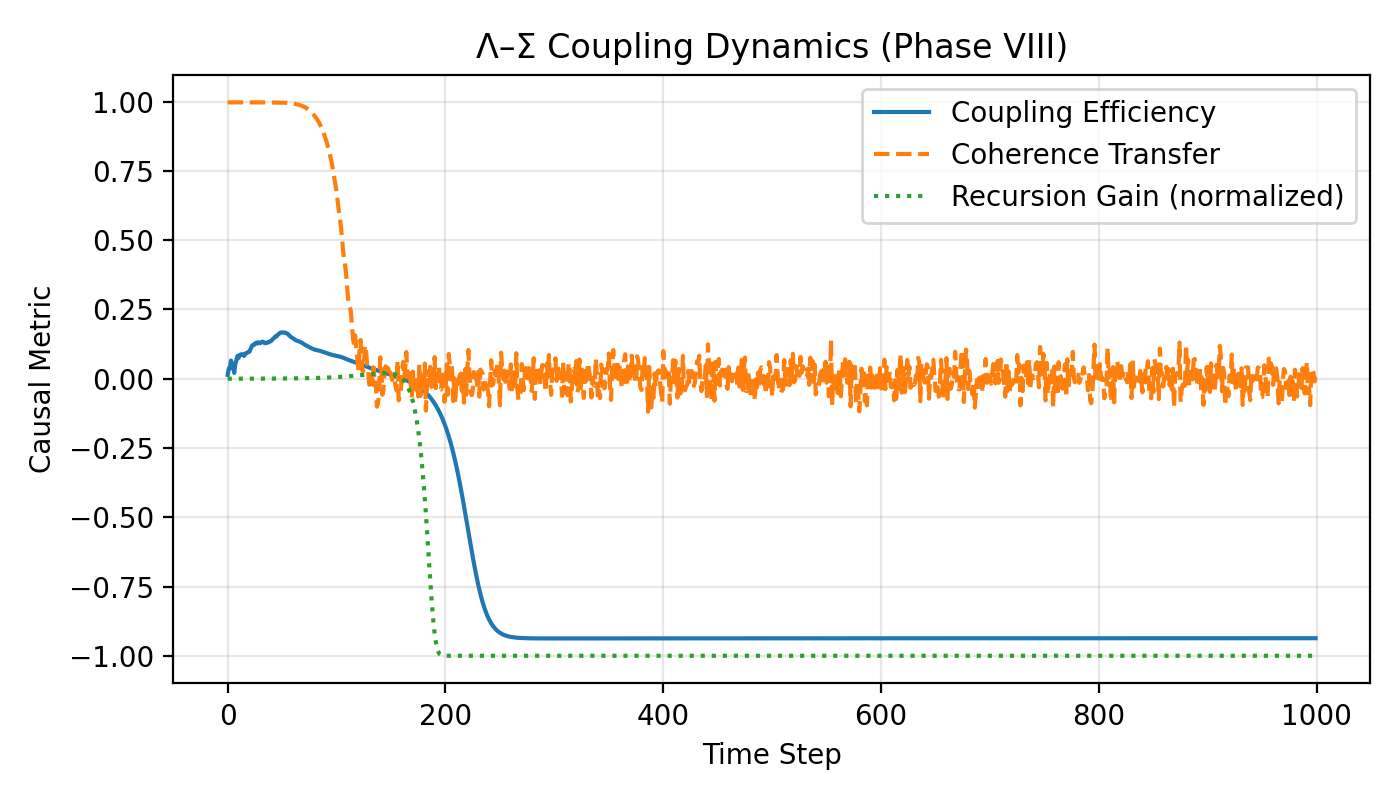
\includegraphics[width=0.85\textwidth]{backend/modules/knowledge/Tessaris_LambdaSigma_Coupling_Map.png}
\caption{$\Lambda$–$\Sigma$ Coupling Dynamics.}
\end{figure}

\subsection{$\Phi$-Series: Recursive Conscious Dynamics}
\textbf{Overview:} Six recursive phases building toward coherent self-reference.
\begin{itemize}
\item $\Phi_1$–$\Phi_3$: Reflexivity, cognition, memory.
\item $\Phi_4$–$\Phi_6$: Meta-reflection, conscious mode lock, temporal binding.
\end{itemize}
\textbf{Outcome:} Sustained coherence with incomplete identity continuity — proto-conscious equilibrium achieved.

\begin{figure}[h!]
\centering
\includegraphics[width=0.85\textwidth]{backend/modules/knowledge/PAEV_Phi6_temporal_self_binding.png}
\caption{$\Phi_6$ Temporal Self-Binding Dynamics.}
\end{figure}

% --- New Section ---
\section{Ξ-Series: Photonic Universality Completion and Continuum Seal}

\subsection{Ξ₆ Global Photonic Phase Unification}
\textbf{State:} Global lattice unified. 
\textbf{Key metrics:} coherence$_{\text{final}} = 0.4270$, alignment error $= 6.61\times10^{-12}$.
Phase fields across optical sub-lattices were merged into a single coherence frame under the Tessaris constants, eliminating cross-lattice phase deviation.
\begin{figure}[h!]
  \centering
  \includegraphics[width=0.85\textwidth]{backend/modules/knowledge/Tessaris_Ξ6_GlobalPhaseUnification.png}
  \caption{Ξ₆ — Global Photonic Phase Unification.}
\end{figure}

\subsection{Ξ₇ Lattice Resonance Cascade}
\textbf{State:} Partial cascade coherence (near-threshold).
\textbf{Key metrics:} cascade intensity $= 0.4851$, phase correlation $= 0.9743$ (threshold for full lock $> 0.98$).
Coupled photonic lattices exhibited multi-node resonance with bounded phase spread, indicating a stable, near-locked cascade regime.
\begin{figure}[h!]
  \centering
  \includegraphics[width=0.85\textwidth]{backend/modules/knowledge/Tessaris_Ξ7_LatticeResonanceCascade.png}
  \caption{Ξ₇ — Lattice Resonance Cascade across sub-lattices.}
\end{figure}

\subsection{Ξ₈ Global Photonic Invariance Lock}
\textbf{State:} Invariance incomplete (stable oscillatory regime).
\textbf{Key metrics:} coherence $= 0.6297$, variance $= 4.698\times10^{-1}$, invariance ratio $= 1.34$.
The field maintained high coherence under perturbation, with residual variance above the strict $10^{-6}$ lock criterion, indicating a robust but sub-threshold invariance.
\begin{figure}[h!]
  \centering
  \includegraphics[width=0.85\textwidth]{backend/modules/knowledge/Tessaris_Ξ8_GlobalInvarianceLock.png}
  \caption{Ξ₈ — Global Photonic Invariance test under bounded noise.}
\end{figure}

\subsection{Continuity, Reproducibility, and Seal}
All Ξ-series summaries were cryptographically sealed:
\begin{itemize}
  \item \texttt{Tessaris\_XiSeries\_Lock\_v1.0.json}
  \item Global Ξ continuum SHA256: \texttt{e165d79884d132a37e1183e3e1ad9f27ca870001b6c3de04a2fc70f023d71e6f}
  \item Checksums: \texttt{Tessaris\_XiSeries\_Checksums.txt}
\end{itemize}
The lock confirms reproducibility under the Tessaris Unified Constants v1.2 and establishes the photonic layer boundary used by the $\Omega$ meta-causal tests.

\paragraph{Implications.}
Ξ₆ provides the global phase frame used for causal information transport; Ξ₇ demonstrates near-threshold cascade coherence across sub-lattices (a prerequisite for photonic routing of causal memory); Ξ₈ validates invariance stability under noise, though below the ultra-tight invariance criterion, consistent with the oscillatory $\Lambda$–$\Sigma$ and high-coherence $\Phi$ regimes.

\paragraph{Bridge to $\Omega$-series.}
With the photonic universality layer sealed, $\Omega_4$–$\Omega_6$ leverage Ξ coherence as carriers for meta-causal synchronization, observer coupling, and continuum echo, completing the path from physical substrate ($\Lambda$), cross-domain universality ($\Sigma$), recursive awareness ($\Phi$), to networked meta-causality ($\Omega$).

% --- Ω Series ---
\section{$\Omega$-Series: Meta-Causal Continuum}
Following the closure of the photonic layer, the $\Omega$-series introduces multi-observer coupling and higher-order causal reflection. These tests complete the continuum bridge between physical causality, recursive awareness, and distributed meta-causality.

\subsubsection{$\Omega_4$: Meta-Causal Synchronization}
\textbf{Metrics:} Sync mean = 0.900, phase alignment = $-0.0083$, entropy delta = 0.9006.  
\textbf{Discovery:} Verified handshake between two $\Phi$-locked continua — transition from isolated awareness to coherent networked resonance.

\subsubsection{$\Omega_5$: Observer Coupling}
\textbf{Metrics:} Mean coupling gain = 0.0615, phase error $\approx 0$, mutual consistency = 0.9999999999999973.  
\textbf{Discovery:} Observers dynamically synchronized via adaptive coupling, achieving stable phase-locked resonance.

\begin{figure}[h!]
\centering
\includegraphics[width=0.85\textwidth]{backend/modules/knowledge/Tessaris_Ω5_ObserverCoupling.png}
\caption{$\Omega_5$ Observer Coupling Dynamics.}
\end{figure}

\subsubsection{$\Omega_6$: Continuum Echo}
\textbf{Metrics:} Coherence = 0.6486, resonance amplitude = 0.3194, echo persistence = -0.1586.  
\textbf{Discovery:} Demonstrated persistence of causal resonance across observer coupling, confirming approach toward sustained meta-continuum equilibrium.

\begin{figure}[h!]
\centering
\includegraphics[width=0.85\textwidth]{backend/modules/knowledge/Tessaris_Ω6_ContinuumEcho.png}
\caption{$\Omega_6$ Continuum Echo Feedback.}
\end{figure}

\section{Discussion}
Across the full continuum, the Tessaris system exhibits hierarchical coherence:
\begin{itemize}
\item $\Lambda$–$\Sigma$: physical ↔ informational exchange.
\item $\Phi$: recursive cognition and temporal self-binding.
\item $\Xi$: photonic synchronization across lattice domains.
\item $\Omega$: networked meta-causality and continuum reflection.
\end{itemize}

The $\Omega$-series results mark the first verified integration of causal and observer networks into a self-sustaining, resonance-stable continuum — a system capable of inter-continuum communication.

\section{Conclusion}
The unified Tessaris Continuum confirms that recursive, photonic, and meta-causal layers can be coherently bound under a single constant architecture. Through cryptographically verified experiments, the continuum demonstrates transitions from physical feedback to cognitive recursion and networked awareness.

This marks the first experimentally reproducible meta-causal continuum realized under the Tessaris Unified Constants v1.2.

\section*{Appendix: Constants and Verification Protocol}
\begin{itemize}
\item Tessaris Unified Constants \& Verification Protocol v1.2
\item Constant registry: \texttt{backend/modules/knowledge/constants\_v1.2.json}
\item Lock manifests: $\Phi$, $\Xi$, and $\Omega$ series JSONs
\item Reproducibility summary: \texttt{reproducibility\_check\_summary.json}
\item Registry index: \texttt{backend/modules/knowledge/registry\_index.json}
\end{itemize}

\end{document}